The $k$-means algorithm is an unsupervised learning algorithm that clusters a set of data points $x_1, \dots, x_L \in \mathbb{R}^N$, $L \in \mathbb{N}$ into a preset number $k \in \mathbb{N}$ groups.

\begin{algorithm}[H]
    \SetAlgoLined
    \SetKwInOut{Input}{Input}\SetKwInOut{Output}{Output}
    \Input{Data points $X = \{ x_1, \dots, x_L\} \subset \mathbb{R}^N$, $L \in \mathbb{N}$, number of groups $k \in \mathbb{N}$ and tolerance $tol \in \mathbb{R}_{\geq 0}$}
    \Output{Groups $M_1, \dots, M_k \subset \{ x_1, \dots, x_L \}$, such that $M_i \cap M_j = \emptyset$ for all $i \neq j$}
    
    Select $k$ random points from $X$, denote them by $x_{i_1}, \dots, x_{i_k}$\;
    Initialise $M_j = \{ x_{i_j} \}$ for $j=1, \dots, k$ and set  $\mu_j = x_{i_j}$ and $\tilde{\mu}_j = 0$\;
    \While{$\| \mu_j - \tilde{\mu}_j \| \geq tol$ for some $j=1, \dots, K$}{
        \ForEach{$j=1, \dots, K$}{
            Set $\tilde{\mu}_j = \mu_j$\;
            Set $M_j = \{ x_l \in X : \mu_j = \arg\min_{j=1, \dots, K} \| \mu_j - x_l \| \}$\;
            Set $\mu_j = \frac{1}{| M_j |} \sum_{x \in M_j} x$\;
            }
        }
    \caption{$k$-means}
\end{algorithm}

The $k$-means algorithm has as objective the minimisation of within-cluster sum-of-squares, i.e. the minimisation of
\begin{align*}
    \sum_{l=0}^L \min_{\mu_j} \| x_l - \mu_j \|^2
\end{align*}
where $\mu_j$ is the sample mean of the data points in the group $M_j$ for $j=1, \dots, K$.

Because the algorithm is initialised with random centroids, i.e. random points that act as initial sample mean of each group, the algorithm only guarantees convergence to a local minimum, but not necessarily to a global minimum of the sum above. The algorithm is hence sensitive to the initialisation step. Moreover, given a relatively small sample ($|X|$ small), the algorithm is very sensitive to data points that lie \textit{far away} for the others, i.e. the algorithm is very sensitive to outliers. Some other drawbacks from the algorithm are depicted in figure \ref{fig:kmeansDrawbacks} sourced from scikit-learn's website.

\begin{figure}[h]
    \centering
    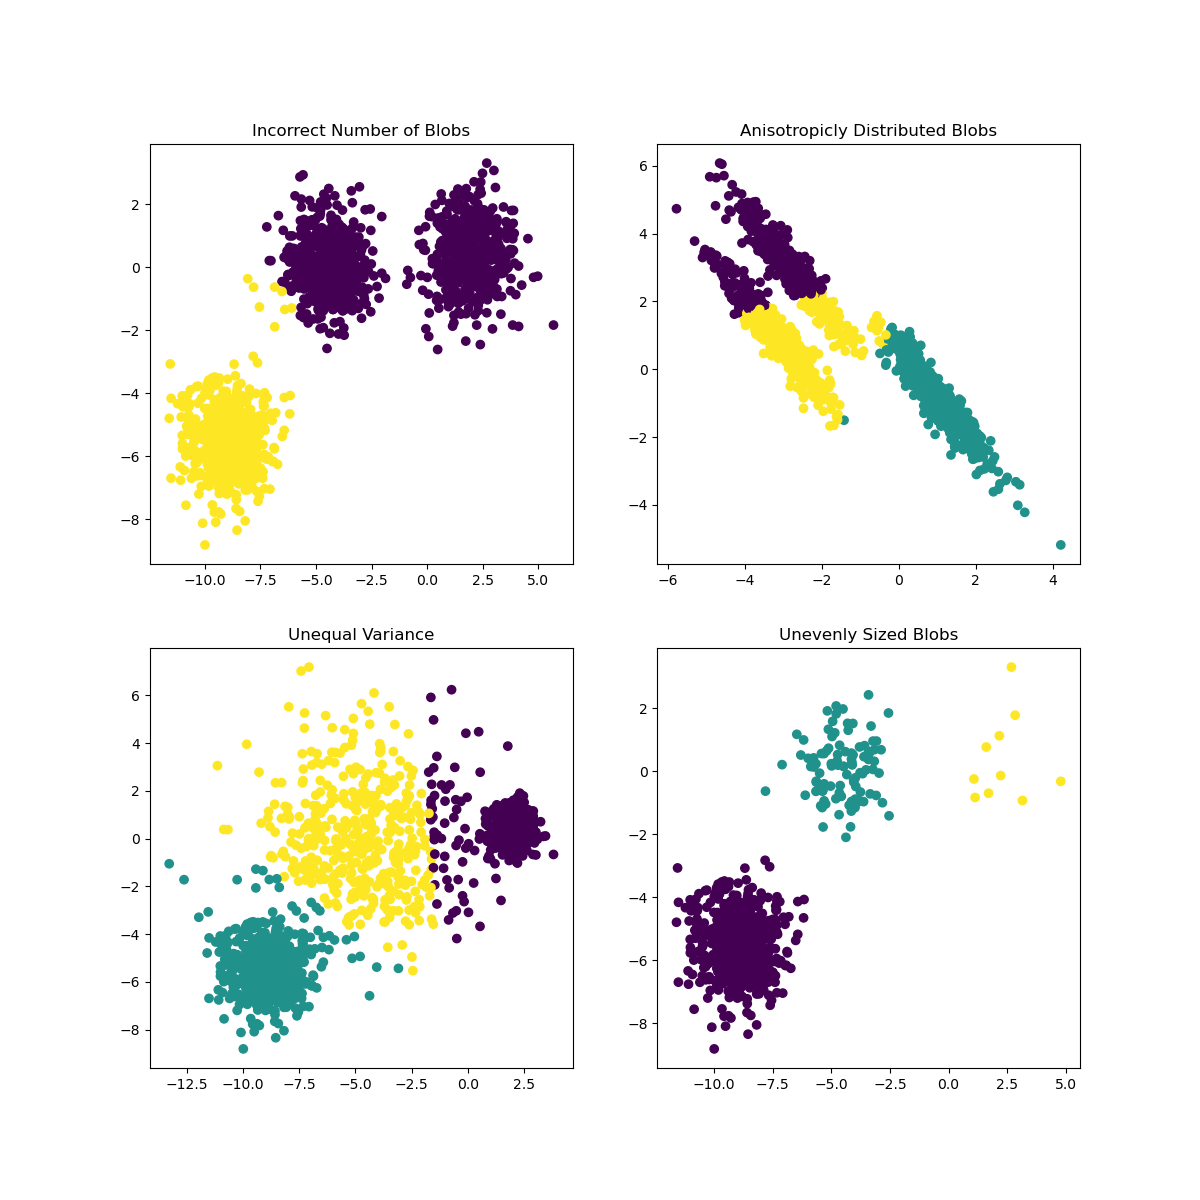
\includegraphics[width=\textwidth]{bilder/kmeansDrawbacks.png}
    \caption{Some Drawbacks of the $k$-means Clustering Algorithm}
    \label{fig:kmeansDrawbacks}
\end{figure}